\section{Interface}

\subsection{Introduction}

J'ai réalisé l'interface principalement sur base de l'usecase et overview diagram ainsi que les choix effectués concernant la base de données et le class diagram.

\begin{flushleft}
Cette manière de procéder m'a permis de structurer mes idées afin de fournir l'interface la plus intuitive possible.
\end{flushleft}

\begin{flushleft}
De plus, il me semblait plus judicieux de n'inclure que la partie qui diffère de l'interface de base afin de permettre une meilleure lisibilité.
\end{flushleft}

\begin{flushleft}
Les \textbf{parties} suivantes seront donc \textbf{conservées} même si elles ne sont pas affichées dans le pdf lié :
\end{flushleft}

\begin{enumerate}[1.]
\item Le système de logs
\item L'interface fournisseur
\item La partie "Contrats" de l'interface client.
\item La partie "Notifications" de l'interface client.
\item La partie "Paramètres" de l'interface client.
\end{enumerate}

\begin{flushleft}
\textbf{Les nouvelles parties} pour l'interface client sont donc essentiellement les suivantes :
\end{flushleft}

\begin{enumerate}[1.]
\item Les portefeuilles "invités"
\item Les clients invités
\end{enumerate}

\begin{flushleft}
Il est important de noter que le logiciel utilisé pour réaliser cette maquette est "Figma".
\end{flushleft}
\newpage

\subsection{L'interface client}

Lorsqu'un client se connectera, il arrivera sur la page d'accueil ou plus précisément "Home" comme sur l'interface de base.
\begin{flushleft}
Ce dernier aura alors les mêmes possibilités ainsi qu'une nouvelle :
\end{flushleft}
\begin{enumerate}
\item Voir ses portefeuilles ("Wallets")
\item Voir les portefeuilles où il est invité ("Invited wallets")
\item Voir ses contrats ("Your contracts")
\item Voir ses notifications
\item Voir les fournisseurs et contrats relatifs ("See new contracts")
\item Se déconnecter
\item Aller sur la page des paramètres
\end{enumerate}

\begin{flushleft}
Il est important de noter que ce n'est qu'à partir de ces sept pages que le client pourra revenir sur la page "Home" étant donné le choix effectué dans mon overview diagram.
\end{flushleft}

\begin{flushleft}
Néanmoins, ce dernier aura la possibilité de revenir en arrière à l'aide du bouton "Back" lorsqu'il sera sur des "sous-pages" de ces sept sections principales.
\end{flushleft}

\newpage

\begin{flushleft}
Commençons par expliquer les modifications survenues pour l'option \textbf{voir ses portefeuilles} ("Wallet").
\end{flushleft}
\begin{flushleft}
Vous pouvez constater l'ajout d'un \textbf{bouton "See guests"} lorsque le client souhaitera voir un portefeuille plus en détail.
\end{flushleft}
\begin{flushleft}
Ce dernier l'emmènera sur une \textbf{page "Guests"} où le client pourra voir la liste des clients qu'il a invités sur chaque portefeuille.
\end{flushleft}
\begin{flushleft}
Cette liste reprendra :
\end{flushleft}

\begin{enumerate}
\item Le nom du client invité
\item Le portefeuille où il est invité
\end{enumerate}

\begin{flushleft}
En outre, le client propriétaire pourra rechercher un client invité en inscrivant son nom ou son adresse mail.
\end{flushleft}

\begin{flushleft}
Le bouton \textbf{"add guests"} le mènera à une page fonctionnant de la même manière que celle contenant la liste d'invités.
\end{flushleft}

\begin{flushleft}
En effet, il pourra rechercher un client à inviter à l'aide de  son nom ou son adresse mail et devra séléctionner un (seul) portefeuille avant de cliquer sur \textbf{le bouton "ADD"} pour ajouter ce nouvel invité à un de ses portefeuilles.
\end{flushleft}

\begin{flushleft}
Ce bouton est relié à la page "Choose permissions" permettant à un client propriétaire de choisir les permissions qu'il souhaite associer à un client. 
\end{flushleft}

\begin{flushleft}
Le bouton "Choose" validera l'ajout du client avec ses permissions.
\end{flushleft}

\begin{flushleft}
Si nous revenons à la liste des clients invités expliquée précédemment, vous pouvez apercevoir également un \textbf{bouton "Go"}. 
\end{flushleft}

\begin{flushleft}
Ce dernier permet de voir plus en détail le client invité :
\end{flushleft}

\begin{enumerate}
\item Le nom du client invité
\item Le portefeuille où il est invité
\item Ses permissions
\end{enumerate}

\begin{flushleft}
Sur cette même page, le client propriétaire aura la possibilité de voir le portefeuille associé concerné en détail (bouton "See" menant à son portefeuille), de retirer son invité de ce dernier (bouton "Delete from this wallet") ainsi que de changer ses permissions (Bouton "Change" menant à la page "Choose permissions").
\end{flushleft}


\newpage

\begin{flushleft}
Nous pouvons maintenant passer à notre nouvelle section \textbf{"Invited Wallets"}.
\end{flushleft}
\begin{flushleft}
Cette page affichera de la même façon que la page "Wallet" une liste des portefeuilles où le client est invité.
\end{flushleft}
\begin{flushleft}
La seule différence réside dans le fait qu'il ne pourra pas ajouter de portefeuilles par lui-même et qu'il peut voir ses permissions.
\end{flushleft}
\begin{flushleft}
Ce dernier doit attendre une invitation dans ses notifications par le client propriétaire.
\end{flushleft}

\begin{flushleft}
Le bouton "Go" le mènera sur une page montrant en détail le portefeuille comme pour le client propriétaire sans oublier ses permissions.
\end{flushleft}

\begin{flushleft}
Remarquez que lorsque le client cliquera sur le bouton "Go" permettant de voir plus en détail les contrats, il n'aura pas le droit de supprimer un contrat lié.
\end{flushleft}

\begin{flushleft}
En cliquant sur le \textbf{bouton "Consumptions"}, le client pourra soit intéragir avec les consommations de la même manière qu'un gestionnaire en cas de "Read and write" c'est à dire qu'il pourra ajouter et changer des données de consommation, soit il n'aura pas accès à ses options mais pourra uniquement visualiser les données en cas de "Read only".
\end{flushleft}

\begin{flushleft}
Il est important de préciser que le niveau d'accès :
\end{flushleft}\begin{enumerate}
\item Read only
\item Read and write
\item Management (pour un client propriétaire)
\end{enumerate}
\begin{flushleft}
est indiqué en haut de chaque page concernant la gestion de données de consommation.
\end{flushleft}

\newpage
\begin{figure}[h]
\subsection{Image de l'interface}
\centering
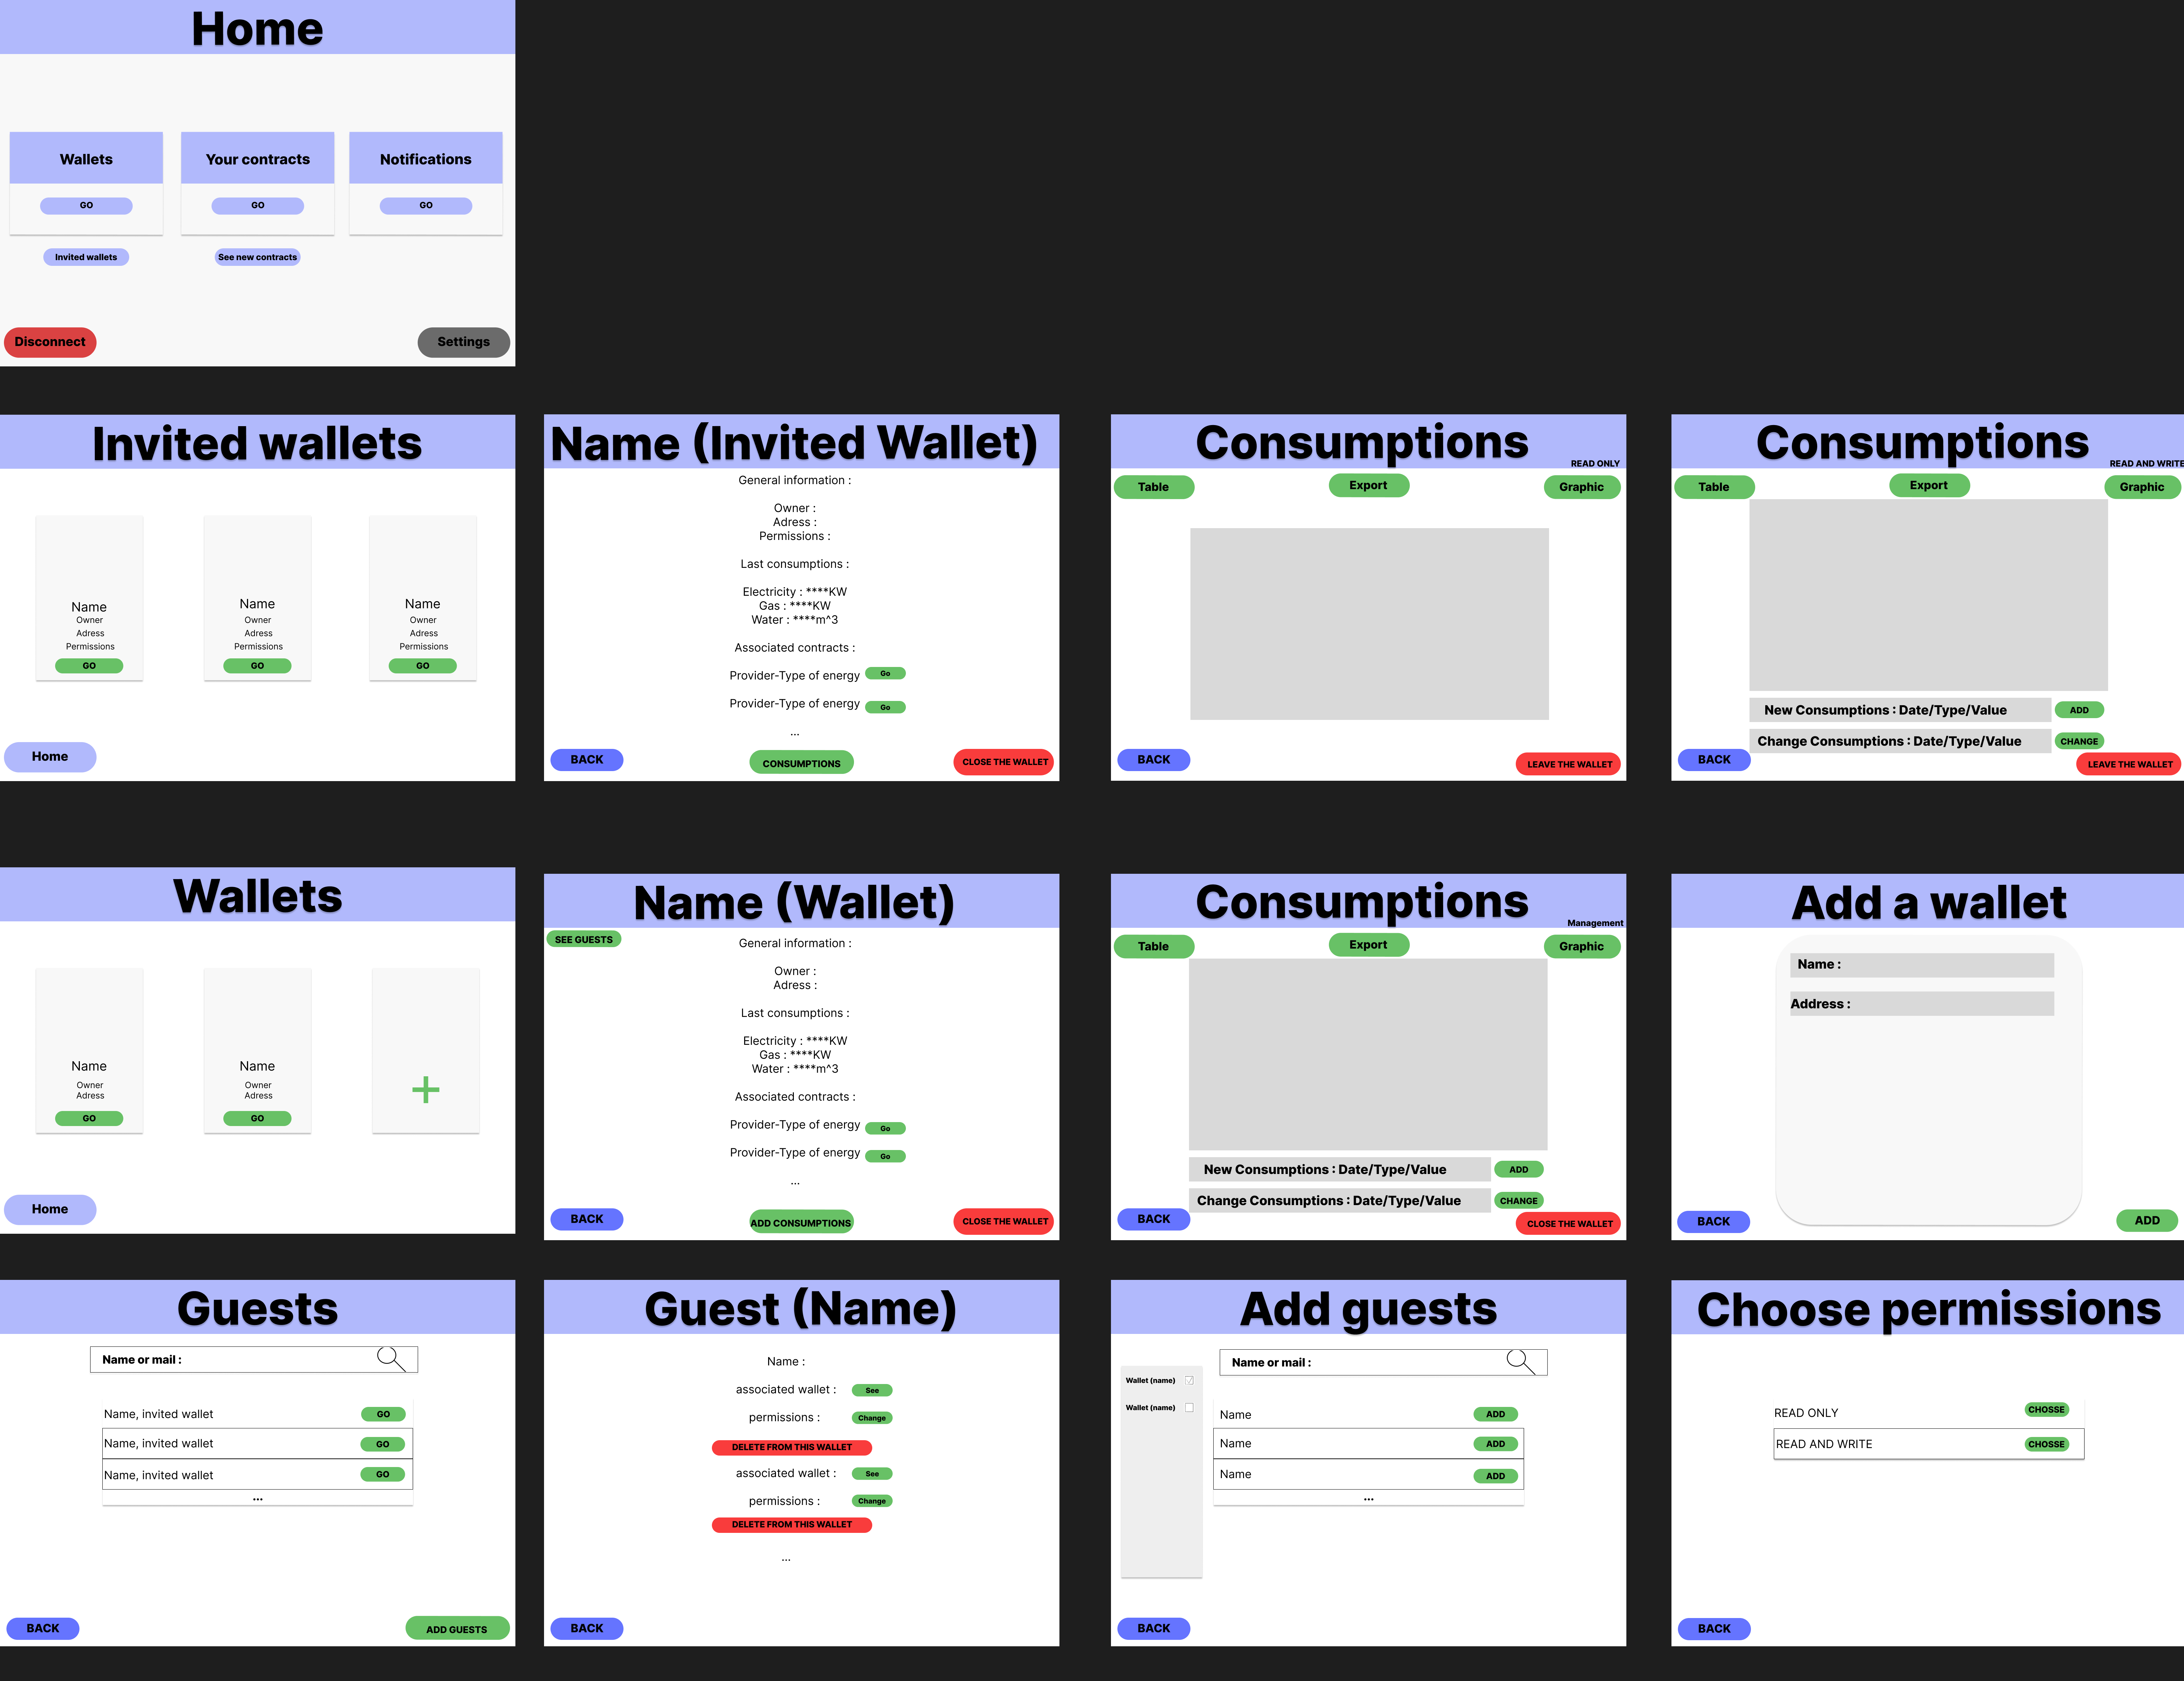
\includegraphics[width = 1\textwidth]{Extension-claire/Interface-claire/img/MonInterface.png}
\end{figure}